\documentclass[11pt]{article}

% This file will be kept up-to-date at the following GitHub repository:
%
% https://github.com/alexhernandezgarcia/latex-simple
%
% Please file any issues/bug reports, etc. you may have at:
%
% https://github.com/alexhernandezgarcia/latex-simple/issues

% With no package options, the submission will be anonymized, the supplemental
% material will be suppressed, and line numbers will be added to the manuscript.
%
% To hide the supplementary material (e.g., for the first submission deadline),
% use the [hidesupplement] option:
%
% \usepackage[hidesupplement]{latex-simple}
%
% To compile a non-anonymized camera-ready version, add the [final] option (for
% the main track) e.g.,
%
% \usepackage[final]{latex-simple}
%
% or
%
% \usepackage[final, hidesupplement]{latex-simple}

\usepackage[final]{latex-simple}

% You may use any reference style as long as you are consistent throughout the
% document. As a default we suggest author--year citations; for bibtex and
% natbib you may use:

\usepackage{natbib}

% and for biber and biblatex you may use:

% \usepackage[%
%   backend=biber,
%   style=authoryear-comp,
%   sortcites=true,
%   natbib=true,
%   giveninits=true,
%   maxcitenames=2,
%   doi=false,
%   url=true,
%   isbn=false,
%   dashed=false
% ]{biblatex}
% \addbibresource{...}

% AMS math
\usepackage{amsmath}
\usepackage{amsthm}

% Dummy text
\usepackage[english]{babel}
\usepackage{blindtext}

% Other packages
\usepackage{microtype} % microtypography
\usepackage{booktabs}  % tables
\usepackage{url}  % urls
\usepackage{titlesec}
\usepackage{setspace}
\usepackage{graphicx}
\graphicspath{{figures/}}
\usepackage{float}
\usepackage{subcaption}
\usepackage{caption}
\usepackage[hidelinks]{hyperref}
\usepackage{booktabs}

% Pour le diagramme de l'architecture
\usepackage{xcolor}
\usepackage{tikz}
\usetikzlibrary{arrows.meta, positioning, fit, backgrounds, calc}
\usepackage{float}  % pour [H]
%%%%%%%%%
% TITLE %
%%%%%%%%%

\title{Segmentation de glaciers alpins à l'aide d'Attention U-Net sur des images satellites}

%%%%%%%%%%%
% AUTHORS %
%%%%%%%%%%%

% The syntax for adding an author is
%
% \author[i]{\nameemail{author name}{author email}}
%
% where i is an affiliation counter. Authors may have
% multiple affiliations; e.g.:
%
% \author[1,2]{\nameemail{Anonymous}{anonymous@example.com}}

\author[1]{\nameemail{Pierre Emery}{pierre.emery@umontreal.ca}}
\author[1]{\nameemail{Mohamed Atmani}{mohamed.atmani@umontreal.ca}}
\author[1]{\nameemail{Fatou Ndao}{fatou.ndao@umontreal.ca}}

% if you need to force a linebreak in the author list, prepend an \author entry
% with \\:

% \author[3]{\\\nameemail{Author 5}{email5@example.com}}

% Specify corresponding affiliations after authors, referring to counter used in
% \author:

\affil[1]{Université de Montréal}
%%%%%%%
% PDF %
%%%%%%%

% define PDF metadata, please fill in to aid in accessibility of the resulting PDF
\hypersetup{%
  pdfauthor={Pierre Emery, Mohamed Atmani, Fatou Ndao},
  pdftitle={Segmentation de glaciers alpins à l'aide d'Attention U-Net sur des images satellites},
  pdfsubject={Segmentation sémantique d'images satellites Sentinel-2 pour la cartographie glaciaire},
  pdfkeywords={segmentation sémantique, U-Net, Attention Gates, Sentinel-2, GLIMS, glaciers, télédétection, apprentissage profond}
}

%%%%%%%%%
% PAPER %
%%%%%%%%%

\begin{document}
 
\maketitle
 
% petit plan
% abstract + intro page 1
% revue page 2
% methode page 3-4-5
% resultats page 6-7
% conclusion-perspective 8
% contributions des membres + utilisation dun llm 9
 
\begin{abstract}
 La fonte accélérée des glaciers alpins menace l'approvisionnement en eau potable, l'irrigation et la production hydroélectrique de régions entières, et augmente les risques de crues glaciaires et d'effondrements en aval. Suivre leur évolution de manière automatisée et précise permet d'anticiper ces impacts. Ce travail propose un pipeline complet de segmentation supervisée de l'étendue glaciaire à partir d'images Sentinel-2 et des contours GLIMS, incluant un score de qualité pour filtrer les scènes affectées par les nuages, les ombres et la neige saisonnière. Un modèle U-Net avec Attention Gates entraîné sur des glaciers du Caucase atteint un IoU de test de 0{,}83 (0{,}82 sur les Alpes, 0{,}84 sur les Andes), démontrant une capacité de généralisation inter-régions. Nous comparons plusieurs stratégies de régularisation ainsi qu'un modèle alternatif (DeepLabV3+), et montrons que notre U-Net, 5$\times$ plus léger, atteint des performances supérieures au modèle pré-entraîné.
\end{abstract}
 
\section{Introduction}
 
Les glaciers constituent des indicateurs particulièrement sensibles du changement climatique. Leur recul accéléré au cours des dernières décennies a des conséquences concrètes : modification des régimes hydrologiques alimentant l'eau potable, l'irrigation et l'hydroélectricité, perturbation des écosystèmes de montagne, et augmentation de certains risques naturels tels que la formation de lacs glaciaires instables ou les crues soudaines. Suivre leur évolution de manière automatisée et précise est donc essentiel pour anticiper et gérer ces impacts.
 
L'imagerie satellitaire, en particulier le programme Sentinel-2~\citep{drusch2012sentinel}, offre aujourd'hui une couverture régulière et à haute résolution de la surface terrestre, ouvrant la voie à des approches d'apprentissage automatique pour la cartographie glaciaire. Parallèlement, des bases de données telles que GLIMS
(\textit{Global Land Ice Measurements from Space})~%
\citep{raup2007glims} fournissent des contours datés pour des milliers de glaciers à travers le monde, constituant une source de supervision exploitable pour l'entraînement de modèles de segmentation.
 
Ce projet formule la cartographie glaciaire comme une tâche de segmentation binaire supervisée. Il propose un pipeline complet allant de la construction d'un jeu de données avec des masques de supervision, à l'entraînement et l'évaluation de modèles de segmentation supervisée. Nous formulons la tâche comme une segmentation binaire : à partir d'un composite d'images Sentinel-2, le modèle doit prédire un masque distinguant les pixels glaciaires du terrain environnant. Nous nous concentrons en particulier sur deux enjeux pratiques : le contrôle de qualité des scènes satellitaires, qui conditionne toute la chaîne en aval, et la capacité du modèle à généraliser au-delà de la région d'entraînement.
 
%%%%%%%%%%%%%%%%%%%%%%%%%%
% PAGE 2 : REVUE
%%%%%%%%%%%%%%%%%%%%%%%%%%
 
\pagebreak
\section{Revue de la littérature}
\input{revue}
 
%%%%%%%%%%%%%%%%%%%%%%%%%%
% PAGES 3-4 : METHODE
%%%%%%%%%%%%%%%%%%%%%%%%%%
 
\pagebreak
\section{Jeu de données}
 
Notre pipeline comporte trois étapes : le nettoyage des contours GLIMS, la récupération et le filtrage des images Sentinel-2, puis la rastérisation des polygones en masques binaires.
 
Les outlines de GLIMS Glacier Database constituent notre source de supervision, mais nécessitent un nettoyage préalable pour apparier les données avec les images satellites utilisées. Nous conservons uniquement les outlines datés entre 2016 et 2026 puisque nous utilisons exclusivement des produits Sentinel-2 L2A, disponibles depuis 2019, période à partir de laquelle
l'ESA produit systématiquement le niveau L2A avec une couche SCL
fiable. Les doublons et entrées redondantes sont supprimés, et seuls les champs d'identification et de géométrie sont retenus. Pour les images satellites, le modèle prend en entrée 5 bandes spectrales : Blue, Green, Red, NIR et SWIR16. Les bandes de proche infrarouge et infrarouge à courte ondes permettent de séparer glacier, eau et roche grâce à leurs réponses spectrales distinctes. 
 
\subsection{Analyse de qualité et sélection des scènes}
La majorité des scènes récupérées étaient initialement inexploitables
en raison de la neige saisonnière, de nuages ou des ombres couvrant
les glaciers. Pour filtrer les images, nous exploitons la couche \textit{Scene Classification Layer} (SCL) des produits Sentinel-2 L2A et
définissons un score de qualité spatiale :
\[
\mathrm{score}
= w_1 \, f_{\text{cloud, glacier}}
+ w_2 \, f_{\text{shadow, glacier}}
+ w_3 \, f_{\text{snow, ring}}
+ w_4 \, (1 - f_{\text{valid}})
\]
Ce score distingue les pixels à l'intérieur du glacier de ceux dans
une couronne extérieure, pénalisant les nuages et ombres sur le
glacier ainsi que la neige autour (qui brouille les contours). La
neige sur le glacier n'est pas pénalisée, car le SCL classe
la glace permanente comme neige/glace, ce qui créerait un plancher
faussement élevé.

Les scènes sont recherchées dans une fenêtre temporelle étroite de
2 à 3 semaines à la fin de l'été (par exemple mi-septembre à
début octobre pour les Alpes), période où la couverture de neige
saisonnière est minimale et les contours glaciaires sont les plus
visibles. Malgré ce filtrage temporel et le score de qualité, les
meilleures scènes individuelles présentaient fréquemment des nuages
résiduels couvrant partiellement le glacier. Pour y remédier, nous
construisons un composite médian à partir des 3 scènes ayant les
meilleurs scores au sein de cette fenêtre. 

 
\begin{figure}[H]
  \centering
  \begin{subfigure}[t]{0.235\textwidth}\centering
    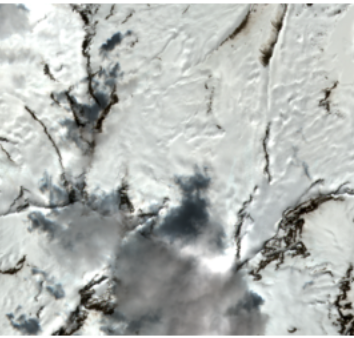
\includegraphics[width=\textwidth]{composite_avant_strategie.png}
    \caption{Avant stratégie}
  \end{subfigure}
  \begin{subfigure}[t]{0.24\textwidth}\centering
    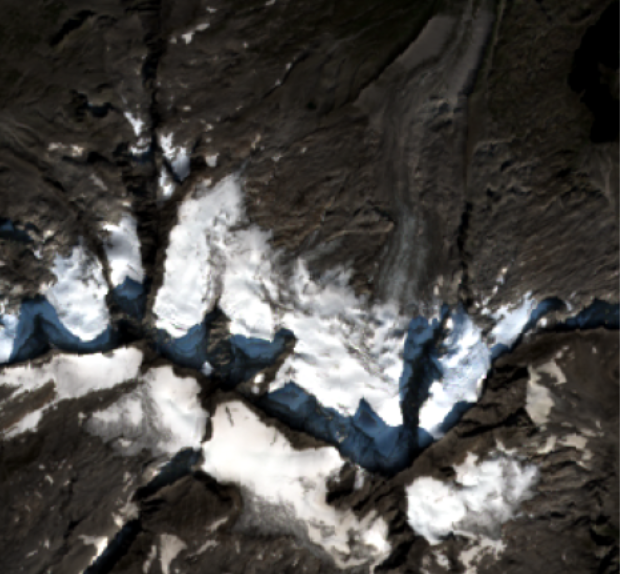
\includegraphics[width=\textwidth]{composite_apres_strategie.png}
    \caption{Après stratégie}
  \end{subfigure}
  \begin{subfigure}[t]{0.24\textwidth}\centering
    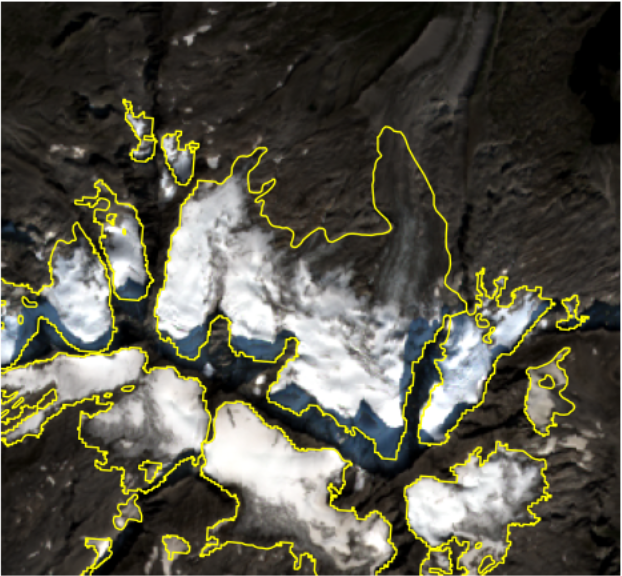
\includegraphics[width=\textwidth]{composite_superposé.png}
    \caption{Superposition avec contours}
  \end{subfigure}
  \begin{subfigure}[t]{0.24\textwidth}\centering
    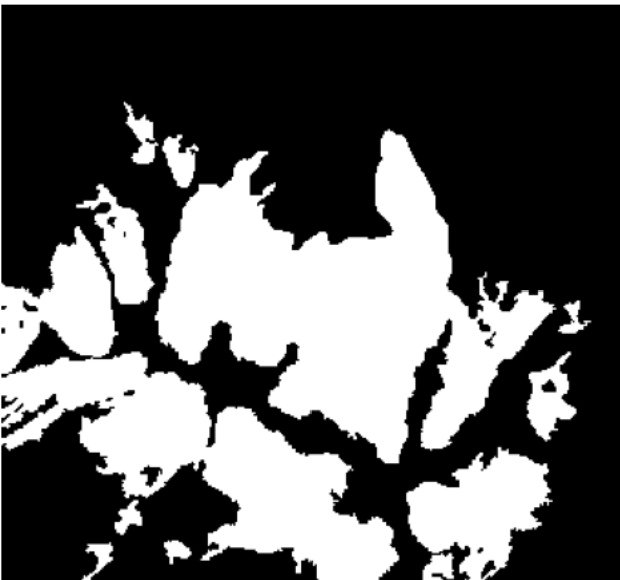
\includegraphics[width=\textwidth]{masque_supervision.png}
    \caption{Masque de supervision}
  \end{subfigure}
  \caption{Construction du jeu de données : différence avant/après la stratégie de sélection et création des masques.}
  \label{fig:quality}
\end{figure}
 

 
\subsection{Rastérisation et création des masques}
Chaque composite est centré sur un glacier principal, sélectionné
parmi les glaciers de surface suffisante ($ \geq 0{,}5$\,km$^2$)
pour lesquels un contour GLIMS daté à moins de 3 ans de l'image
satellite est disponible. Cependant, l'image de $320 \times 320$
pixels capture également les glaciers voisins, pour lesquels le
contour le plus récent peut être plus ancien et donc moins fidèle
à la réalité au moment de l'acquisition. Pour chacun de ces glaciers
secondaires, nous sélectionnons le contour GLIMS le plus proche
temporellement de l'image.

Les polygones GLIMS sont ensuite reprojetés et rastérisés sur la
grille Sentinel-2 pour produire des masques binaires alignés pixel
à pixel, servant pour la supervision de l'apprentissage. Afin de
contrôler la qualité de ces masques, nous affichons chaque composite
avec ses contours superposés et rejetons manuellement les images
pour lesquelles le décalage entre les contours et l'étendue glaciaire
visible est trop important. Au total, le jeu de données retenu compte
582 paires composite-masque réparties sur trois régions.

\subsection{Séparations des ensembles d'entraînement, validation et test}
Pour éviter les fuites d'information, nous adoptons une séparation
par région pour l'entraînement, et une séparation aléatoire sans
chevauchement pour la validation et le test, le dataset final est donc séparé ainsi : entraînement sur le Caucase (346 paires), validation et test sur les Alpes et Andes mélangés (118 paires respectivement). Le split est fixé par une \emph{random seed} et sauvegardé
pour garantir la reproductibilité. Ce protocole permet d'évaluer la
généralisation à des chaînes non vues à l'entraînement : les Alpes
(plus similaire au Caucase) et les Andes (une chaîne différente).

\section{Modèle et choix méthodologiques}

\subsection{Architecture : Attention U-Net}

Nous utilisons un U-Net \citep{ronneberger2015unet} augmenté d'\emph{Attention Gates} \citep{AttentionGates2018} comme modèle principal. Cette architecture encodeur-décodeur est particulièrement adaptée à notre tâche car la segmentation glaciaire requiert à la fois une compréhension sémantique globale (distinguer la glace des nuages, de la neige saisonnière ou de la roche claire) et une précision spatiale au pixel près pour délimiter les contours.


%  Diagramme de l'architecture U-Net (TikZ)

\begin{figure}[H]
\centering
\resizebox{\textwidth}{!}{%
\begin{tikzpicture}[
    font=\small,
    % --- styles des blocs ---
    attn/.style={
        draw, fill=yellow!40, diamond, 
        minimum width=0.4cm, minimum height=0.4cm,
        inner sep=0pt, line width=0.6pt
    },
    conv/.style={
        draw, fill=blue!20, rounded corners=3pt,
        minimum width=1.0cm, minimum height=2.2cm,
        line width=0.7pt
    },
    bottle/.style={
        draw, fill=purple!25, rounded corners=3pt,
        minimum width=1.0cm, minimum height=1.4cm,
        line width=0.7pt
    },
    pool/.style={
        draw, fill=red!15, rounded corners=2pt,
        minimum width=0.35cm, minimum height=2.2cm,
        line width=0.6pt
    },
    up/.style={
        draw, fill=green!15, rounded corners=2pt,
        minimum width=0.35cm, minimum height=2.2cm,
        line width=0.6pt
    },
    head/.style={
        draw, fill=orange!25, rounded corners=3pt,
        minimum width=0.7cm, minimum height=2.2cm,
        line width=0.7pt
    },
    lbl/.style={font=\scriptsize, align=center},
    % --- flèches ---
    arr/.style={-{Stealth[length=4pt]}, line width=0.8pt},
    skip/.style={-{Stealth[length=4pt]}, dashed, line width=0.8pt, color=gray!70},
]

% espacement
\def\dx{1.55}   % entre blocs conv successifs
\def\dxp{0.55}  % largeur pool/up

%encodeur
% enc0  (in=5, out=32)  h=2.2
\node[conv, minimum height=2.2cm] (e0) at (0,0) {};
\node[lbl, above=2pt of e0] {32};

% pool0
\node[pool, right=0.12cm of e0] (p0) {};

% enc1  (out=64)  h=1.8
\node[conv, minimum height=1.8cm, right=0.12cm of p0] (e1) {};
\node[lbl, above=2pt of e1] {64};

% pool1
\node[pool, minimum height=1.8cm, right=0.12cm of e1] (p1) {};

% enc2  (out=128)  h=1.4
\node[conv, minimum height=1.4cm, right=0.12cm of p1] (e2) {};
\node[lbl, above=2pt of e2] {128};

% pool2
\node[pool, minimum height=1.4cm, right=0.12cm of e2] (p2) {};

% enc3  (out=256)  h=1.0
\node[conv, minimum height=1.0cm, right=0.12cm of p2] (e3) {};
\node[lbl, above=2pt of e3] {256};

% pool3
\node[pool, minimum height=1.0cm, right=0.12cm of e3] (p3) {};

%bottleneck
\node[bottle, right=0.12cm of p3] (bn) {};
\node[lbl, above=2pt of bn] {512};
\node[lbl, below=2pt of bn] {Dropout\\(p=0.3)};

% decodeur
% up3
\node[up, minimum height=1.0cm, right=0.12cm of bn] (u3) {};
% dec3  (out=256)  h=1.0
\node[conv, minimum height=1.0cm, right=0.12cm of u3] (d3) {};
\node[lbl, above=2pt of d3] {256};

% up2
\node[up, minimum height=1.4cm, right=0.12cm of d3] (u2) {};
% dec2  (out=128)  h=1.4
\node[conv, minimum height=1.4cm, right=0.12cm of u2] (d2) {};
\node[lbl, above=2pt of d2] {128};

% up1
\node[up, minimum height=1.8cm, right=0.12cm of d2] (u1) {};
% dec1  (out=64)  h=1.8
\node[conv, minimum height=1.8cm, right=0.12cm of u1] (d1) {};
\node[lbl, above=2pt of d1] {64};

% up0
\node[up, minimum height=2.2cm, right=0.12cm of d1] (u0) {};
% dec0  (out=32)  h=2.2
\node[conv, minimum height=2.2cm, right=0.12cm of u0] (d0) {};
\node[lbl, above=2pt of d0] {32};

% (Conv 1×1 → logits)
\node[head, right=0.3cm of d0] (hd) {};
\node[lbl, above=2pt of hd] {Conv\\$1{\times}1$};

% entrée et sortie
\node[lbl, left=0.35cm of e0] (inp) {Entrée\\$320{\times}320$\\5 bandes};
\draw[arr] (inp) -- (e0);

\node[lbl, right=0.35cm of hd] (out) {Masque\\$320{\times}320$\\(logits)};
\draw[arr] (hd) -- (out);

% flèches
\foreach \a/\b in {e0/p0, p0/e1, e1/p1, p1/e2, e2/p2, p2/e3, e3/p3,
                   p3/bn, bn/u3, u3/d3, d3/u2, u2/d2, d2/u1, u1/d1,
                   d1/u0, u0/d0, d0/hd}
    \draw[arr] (\a) -- (\b);


%skip connections
% Calcul des positions y pour les arcs
% enc0 → dec0  (niveau 0, h=2.2)
% enc3 → dec3 (avec Attention Gate)
\node[attn] (ag3) at ($(d3.north)+(0,0.55)$) {};
\draw[skip] (e3.north) to[out=90, in=90, looseness=0.40] (ag3.north);
\draw[arr, color=gray!70] (ag3) -- (d3.north);

% enc2 → dec2 (avec Attention Gate)
\node[attn] (ag2) at ($(d2.north)+(0,0.55)$) {};
\draw[skip] (e2.north) to[out=90, in=90, looseness=0.34] (ag2.north);
\draw[arr, color=gray!70] (ag2) -- (d2.north);

% enc1 → dec1 (avec Attention Gate)
\node[attn] (ag1) at ($(d1.north)+(0,0.55)$) {};
\draw[skip] (e1.north) to[out=90, in=90, looseness=0.30] (ag1.north);
\draw[arr, color=gray!70] (ag1) -- (d1.north);

% enc0 → dec0 (avec Attention Gate)
\node[attn] (ag0) at ($(d0.north)+(0,0.55)$) {};
\draw[skip] (e0.north) to[out=90, in=90, looseness=0.28] (ag0.north);
\draw[arr, color=gray!70] (ag0) -- (d0.north);


%légende
\begin{scope}[shift={(0,-2.2)}]
    \node[conv,   minimum height=0.45cm, minimum width=0.75cm] (le) at (0,0) {};
    \node[lbl, right=0.1cm of le] {DoubleConv (Conv $3{\times}3$ $\to$ BN $\to$ ReLU) $\times 2$};

    \node[pool,   minimum height=0.45cm, minimum width=0.35cm] (lp) at (0,-0.65) {};
    \node[lbl, right=0.1cm of lp] {MaxPool $2{\times}2$};

    \node[up,     minimum height=0.45cm, minimum width=0.35cm] (lu) at (3.5,-0.65) {};
    \node[lbl, right=0.1cm of lu] {ConvTranspose $2{\times}2$};

    \node[bottle, minimum height=0.45cm, minimum width=0.75cm] (lb) at (12,0) {};
    \node[lbl, right=0.1cm of lb] {Bottleneck + Dropout};

    % skip legend
    \draw[skip] (7.2,0) -- (8.0,0);
    \node[lbl, right=0.05cm] at (8.0,0) {Skip connection};
    \node[attn] (la) at (7.2,-0.65) {};
    \node[lbl, right=0.1cm of la] {Attention Gate};
\end{scope}

% labels encodeur/decodeur/bottleneck
\node[lbl, gray, above=0.55cm] at ($(e0)!0.5!(p3)$) {\textsc{Encodeur}};
\node[lbl, gray, above=0.55cm] at ($(u3)!0.5!(d0)$) {\textsc{Décodeur}};
\node[lbl, gray, above=0.55cm] at (bn)              {\textsc{Bottleneck}};


\foreach \n in {p0,p1,p2,p3}
    \node[lbl, rotate=90, font=\tiny, text=red!60!black] at (\n) {MP};
\foreach \n in {u0,u1,u2,u3}
    \node[lbl, rotate=90, font=\tiny, text=green!50!black] at (\n) {CT};

\end{tikzpicture}
}
\caption{Architecture U-Net avec Attention Gates utilisée pour la segmentation glaciaire.}
\label{fig:unet_architecture}
\end{figure}

L'encodeur enchaîne des blocs de double convolution $3{\times}3$ (BatchNorm \citep{BatchNorm2015} + ReLU) et des max-pooling $2{\times}2$, selon la séquence de filtres $[32, 64, 128, 256]$. Le \emph{bottleneck} à 512 filtres inclut un \emph{Dropout} spatial \citep{Dropout2014} ($p=0{,}3$) qui masque des canaux entiers de \emph{feature maps} plutôt que des neurones individuels, ce qui régularise au point de plus forte compression. Le décodeur remonte symétriquement la résolution via des convolutions transposées $2{\times}2$, avec des \textit{skip connections} \citep{SkipConnections2015} qui préservent l'information de localisation perdue par le \emph{pooling}. Avant chaque concaténation, un \emph{Attention Gate} filtre le signal de l'encodeur : le signal du décodeur (sémantiquement riche) guide un masque d'attention appris qui pondère chaque pixel du signal de l'encodeur (spatialement précis), ce qui focalise le décodeur sur les zones glaciaires plutôt que sur le fond. Une convolution $1{\times}1$ finale produit les logits.

Le modèle prend en entrée des patches de 5 bandes Sentinel-2 (B, G, R, NIR, SWIR16) de taille $320{\times}320$ pixels (multiple de $2^4$ imposé par les 4 max-pooling) et produit un masque binaire de même résolution, pour ${\sim}7{,}8$M paramètres entraînables.

\subsection{Modèle de comparaison : DeepLabV3+}

Pour situer les performances de notre U-Net, nous comparons avec DeepLabV3+ \citep{DeepLabV3Plus2018} à \emph{backbone} ResNet50 \citep{ResNet2015} pré-entraîné sur ImageNet. Ce modèle capture le contexte multi-échelle via un module \textit{Atrous Spatial Pyramid Pooling} (ASPP) de convolutions dilatées en parallèle. Avec ses ${\sim}42$M paramètres (environ 5$\times$ plus que notre U-Net) et son pré-entraînement, il représente une référence exigeante.

Pour l'adapter à nos 5 bandes d'entrée, nous remplaçons la première couche convolutive (3 $\to$ 5 canaux) en conservant les poids pré-entraînés pour les canaux RGB et en initialisant les canaux NIR (\emph{near infrared}) et SWIR avec la moyenne des poids RGB existants. La tête de classification est réinitialisée pour la segmentation binaire, puis l'ensemble du modèle est \emph{fine-tuné} sur nos données avec le même protocole que le U-Net, à l'exception du taux d'apprentissage.

\subsection{Fonction de perte et métrique d'évaluation}

Les métriques utilisées sont standard pour les tâches de
segmentation. Pendant l'apprentissage, le modèle optimise une
fonction de perte combinant la \emph{Binary Cross-Entropy} (BCE) et la
\emph{Dice Loss} ; le modèle est ensuite sélectionné et évalué selon
l'\textit{Intersection over Union} (IoU) \citep{IoU2015} :
\[
\mathcal{L} = \mathcal{L}_{\text{BCE}} + \mathcal{L}_{\text{Dice}},
\quad
\mathcal{L}_{\text{Dice}} = 1 - \frac{2\,|P \cap T|}{|P| + |T|},
\quad
\mathrm{IoU} = \frac{|P \cap T|}{|P \cup T|}
\]
Les deux pertes sont complémentaires : la BCE, calculée pixel
par pixel, fournit un gradient dense et bien conditionné qui
stabilise la convergence, tandis que la Dice Loss, calculée
globalement, optimise directement le recouvrement et gère le
déséquilibre de classes fréquent en segmentation glaciaire.
L'IoU pénalise à la fois les faux positifs et les faux négatifs,
et admet une interprétation géographique directe : un IoU de 0,7
signifie que 70\,\% de la surface prédite et de la surface réelle
se recouvrent.

\subsection{Augmentation de données}

Pour réduire le surapprentissage, nous appliquons des augmentations à la volée pendant l'entraînement. À chaque \emph{epoch}, chaque image est transformée aléatoirement par une combinaison indépendante de retournements horizontal et vertical (50\,\% chacun), rotations de 90°/180°/270° (75\,\%), bruit gaussien ($\sigma = 0{,}02$, 50\,\%), et scaling par bande ($\times 0{,}9$ à $\times 1{,}1$, 50\,\%), environ 98\,\% des images subissant au moins une transformation par \emph{epoch}. Les transformations géométriques sont appliquées de manière synchronisée à l'image et au masque. Les rotations arbitraires sont pertinentes pour des images satellite sans orientation privilégiée ; le bruit et le scaling par bande simulent la variabilité atmosphérique et les conditions d'illumination.

\subsection{Hyperparamètres}

L'entraînement utilise AdamW \citep{AdamW2017} avec un taux d'apprentissage initial de $10^{-3}$ réduit à $10^{-6}$ par un \emph{scheduler cosinus}, et un \emph{weight decay} de $10^{-4}$ \citep{decoupledWeight2019}. Le DeepLabV3+ utilise un taux initial plus bas ($5 \times 10^{-4}$) pour ne pas déstabiliser son \emph{backbone} pré-entraîné. Le tableau~\ref{tab:hyperparams} résume la configuration complète.

\begin{table}[h]
\caption{Hyperparamètres d'entraînement.}
\label{tab:hyperparams}
\begin{center}
\begin{tabular}{ll}
\toprule
Hyperparamètre & Valeur \\
\midrule
Filtres encodeur (U-Net)  & $[32,\ 64,\ 128,\ 256]$ \\
Dropout (bottleneck)      & $0{,}3$ \\
Taille des patches        & $320 \times 320$ px \\
Bandes d'entrée           & 5 (B, G, R, NIR, SWIR16) \\
Taille de batch           & 4 \\
Epoch                     & 100 \\
Optimiseur                & AdamW \\
Taux d'apprentissage      & $10^{-3}$ (U-Net) / $5 \times 10^{-4}$ (DeepLabV3+) \\
Scheduler                 & Cosinus ($\to 10^{-6}$) \\
Weight decay              & $10^{-4}$ \\
\bottomrule
\end{tabular}
\end{center}
\end{table}

 
%%%%%%%%%%%%%%%%%%%%%%%%%%
% PAGES 5-6 : RESULTATS
%%%%%%%%%%%%%%%%%%%%%%%%%%
 
\section{Résultats}
Afin d'évaluer l'impact de chaque technique de régularisation et
de comparer les architectures, nous entraînons cinq modèles :
un U-Net sans aucune régularisation comme \textit{baseline},
un U-Net avec \emph{dropout} et \emph{weight decay} mais sans augmentation
(régularisation uniquement au niveau du modèle), un U-Net avec
augmentation mais sans \emph{dropout} ni \emph{weight decay} (régularisation
uniquement par les données), un U-Net combinant les deux
approches, et DeepLabV3+ (ResNet50) comme modèle de référence
pré-entraîné, avec augmentation et \emph{weight decay}. Tous les modèles
sont entraînés pendant 100 \textit{epochs} sur le Caucase, et le
meilleur \textit{checkpoint} (IoU de validation maximal) est
retenu pour l'évaluation sur le \textit{test set}.

\subsection{Courbes d'entraînement}

La figure~\ref{fig:training} montre l'évolution de la perte et de
l'IoU pour une configuration U-Net avec augmentation, qui atteint
un IoU de validation de ${\sim}0{,}80$. L'écart entre les courbes
d'entraînement et de validation traduit un léger surapprentissage,
attribuable à la taille limitée du jeu de données. Cet écart
était sensiblement plus prononcé pour les configurations sans
augmentation, et encore plus marqué pour le DeepLabV3+, dont le
nombre de paramètres (${\sim}42$M) est bien supérieur à la
quantité de données disponibles.
 
\begin{figure}[H]
  \centering
  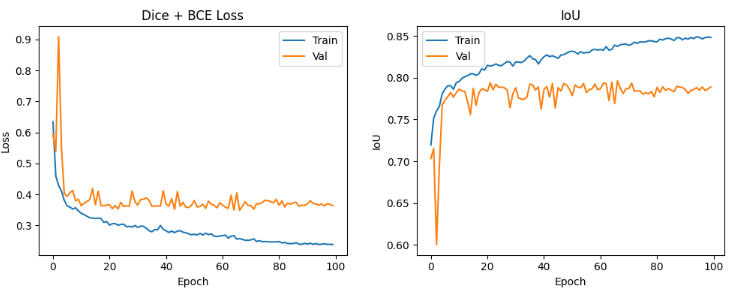
\includegraphics[width=0.8\textwidth]{epoch_vs_loss_final.png}
  \caption{Courbes d'entraînement sur 100 \emph{epoch} (configuration avec augmentation, sans \emph{weight decay} ni \emph{dropout}). Gauche : Dice + BCE Loss. Droite : IoU. }
  \label{fig:training}
\end{figure}
 
\subsection{Étude d'ablation : impact de la régularisation}
Le tableau~\ref{tab:results_global} présente les résultats globaux
sur l'ensemble de test. La \emph{baseline} sans régularisation atteint
déjà $0{,}817$ d'IoU. Le \emph{dropout} et le \emph{ weight decay} seuls
n'apportent pas de gain (et dégradent même légèrement à
$0{,}814$), tandis que l'augmentation de données seule fait
gagner $0{,}7$ point ($0{,}824$). La combinaison des trois
régularisations donne le meilleur résultat ($0{,}830$), suggérant
que le \textit{dropout} et \textit{weight decay} n'apportent un bénéfice additif que
lorsqu'ils sont combinés à l'augmentation.

\begin{table}[H]
\centering
\caption{Résultats sur l'ensemble de test (toutes régions confondues).}
\label{tab:results_global}
\begin{tabular}{lcccccc}
\toprule
\textbf{Modèle} & \textbf{IoU} & \textbf{Dice} & \textbf{Prec.} & \textbf{Recall} & \textbf{F1} & \textbf{Acc.} \\
\midrule
U-Net : baseline (sans rég.)        & 0.8171 & 0.8993 & 0.9105 & 0.8885 & 0.8993 & 0.9172 \\
U-Net : dropout+wd, no aug          & 0.8142 & 0.8976 & 0.9195 & 0.8767 & 0.8976 & 0.9168 \\
U-Net : aug, no dropout/wd          & 0.8242 & 0.9036 & 0.9228 & 0.8852 & 0.9036 & 0.9214 \\
U-Net : aug + dropout + wd          & \textbf{0.8303} & \textbf{0.9073} & 0.9131 & \textbf{0.9015} & \textbf{0.9073} & \textbf{0.9233} \\
\midrule
DeepLabV3+ (ResNet50)               & 0.8128 & 0.8967 & \textbf{0.9259} & 0.8694 & 0.8967 & 0.9167 \\
\bottomrule
\end{tabular}
\end{table}
 
\subsection{Comparaison architecturale : U-Net vs DeepLabV3+}
Le DeepLabV3+ pré-entraîné sur ImageNet (${\sim}42$M paramètres) obtient un IoU de $0{,}813$, inférieur à notre meilleur U-Net ($0{,}830$, ${\sim}7{,}8$M paramètres). Ce résultat s'explique par plusieurs facteurs : (1) le backbone ResNet50 est optimisé pour 3 canaux RGB et des photos naturelles, pas pour des images satellite à 5 bandes --- l'adaptation de la première couche convolutive ne suffit pas à réajuster les représentations profondes en 100 \emph{epochs} ; (2) la capacité supplémentaire du DeepLabV3+ est surdimensionnée pour notre tâche de segmentation binaire relativement simple ; (3) le U-Net, entraîné \emph{
from scratch}, apprend des \emph{features} directement adaptées aux propriétés spectrales des glaciers.
 
\subsection{Résultats par région}
Le tableau~\ref{tab:results_regions} détaille les performances par
région. Un résultat notable est que tous les modèles performent
mieux sur les Andes que sur les Alpes, alors que le Caucase
(\textit{train}) est géographiquement plus proche des Alpes. Cela
s'explique probablement par la taille plus grande des glaciers
andins dans notre dataset.

\begin{table}[H]
\centering
\caption{Comparaison des modèles par région de test.}
\label{tab:results_regions}
\resizebox{\textwidth}{!}{%
\begin{tabular}{llcccccc}
\toprule
\textbf{Modèle} & \textbf{Région} & \textbf{IoU} & \textbf{Dice} & \textbf{Prec.} & 
\textbf{Recall} & \textbf{F1} & \textbf{Acc.} \\
\midrule
\multirow{}{}{U-Net : baseline (sans rég.)}
  & Alpes  & 0.8143 & 0.8976 & \textbf{0.9396} & 0.8592 & 0.8976 & 0.9291 \\
  & Andes  & 0.8195 & 0.9008 & 0.8868 & 0.9153 & 0.9008 & 0.9027 \\
\midrule
\multirow{}{}{U-Net : dropout+wd, no aug}
  & Alpes  & 0.8146 & 0.8978 & 0.9378 & 0.8611 & 0.8978 & 0.9291 \\
  & Andes  & 0.8139 & 0.8974 & 0.9038 & 0.8911 & 0.8974 & 0.9016 \\
\midrule
\multirow{}{}{U-Net : aug, no dropout/wd}
  & Alpes  & 0.8193 & 0.9007 & 0.9420 & 0.8628 & 0.9007 & \textbf{0.9312} \\
  & Andes  & 0.8285 & 0.9062 & 0.9065 & 0.9058 & 0.9062 & 0.9095 \\
\midrule
\multirow{}{}{U-Net : aug + dropout + wd}
  & Alpes  & \textbf{0.8198} & \textbf{0.9010} & 0.9331 & \textbf{0.8709} & \textbf{0.9010} & 0.9307 \\
  & Andes  & \textbf{0.8396} & \textbf{0.9128} & 0.8966 & \textbf{0.9297} & \textbf{0.9128} & \textbf{0.9143} \\
\midrule
\multirow{}{}{DeepLabV3+}
  & Alpes  & 0.8118 & 0.8961 & 0.9326 & 0.8624 & 0.8961 & 0.9276 \\
  & Andes  & 0.8138 & 0.8973 & 0.9199 & 0.8758 & 0.8973 & 0.9033 \\
\bottomrule
\end{tabular}%
}
\end{table}
 
\subsection{Exemple de prédictions}


La figure~\ref{fig:predictions} présente quelques exemples de
prédictions sur l'ensemble de test. Sur cette carte de différence, il faut interpréter les vrai positifs comme de la glace correctement identifiée, les faux
positifs comme des pixels prédits comme glace alors que le masque GLIMS
indique du fond et les faux négatifs comme de la glace manquée par le modèle.
\begin{figure}[H]
  \centering
  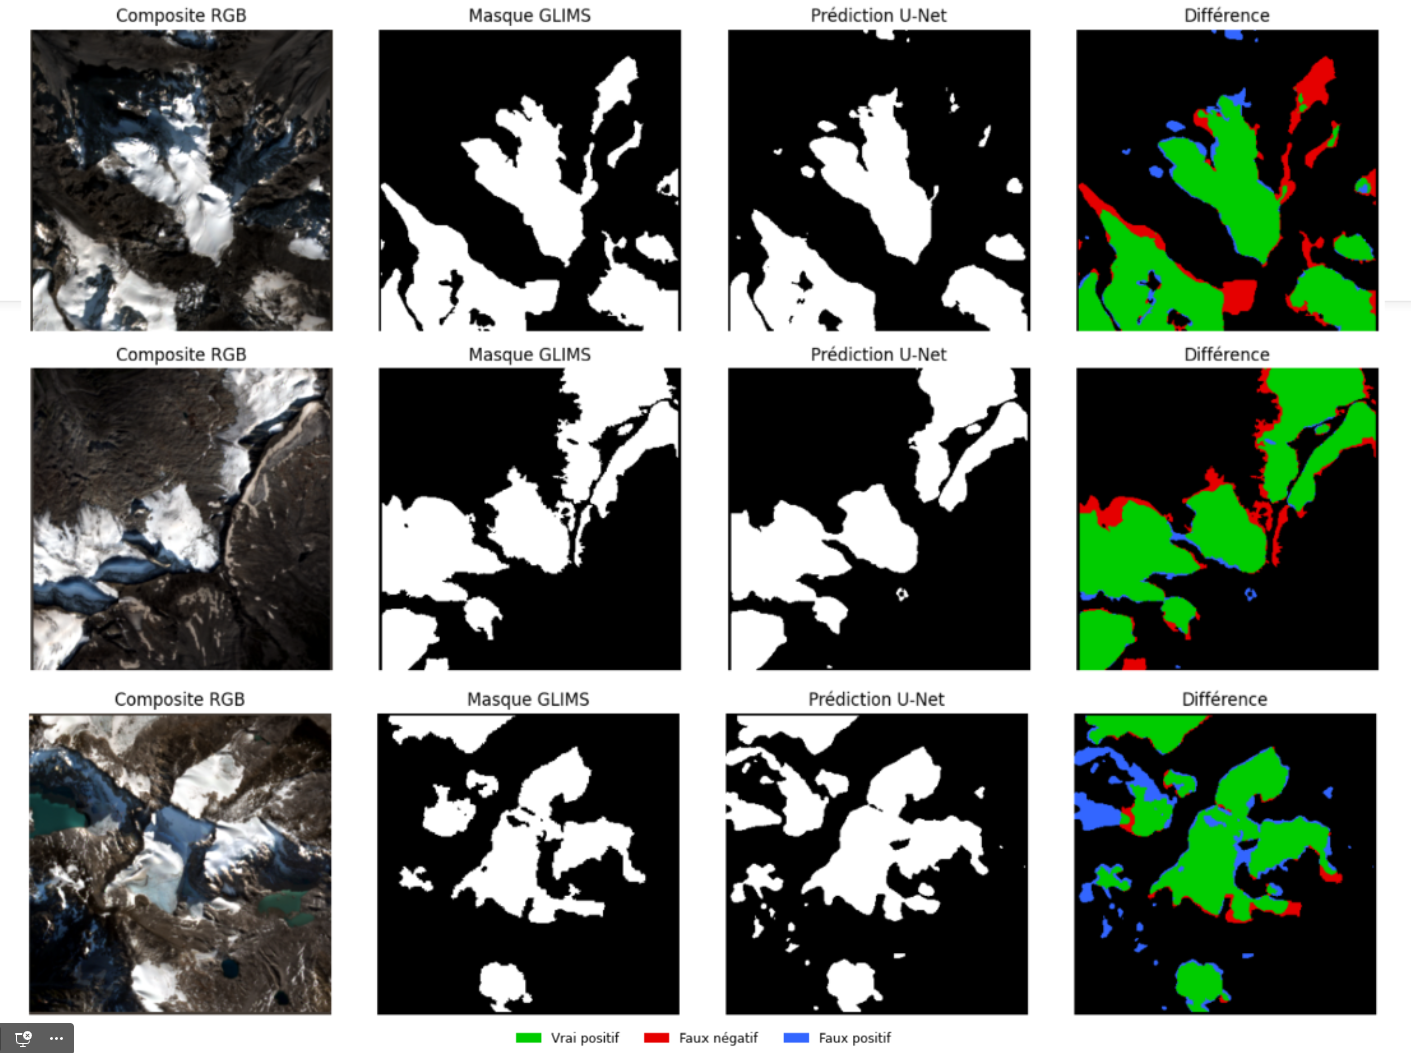
\includegraphics[width=0.9\textwidth]{prediction_unet_final.png}
  \caption{Prédictions sur des composites de test : composite
  Sentinel-2, masque GLIMS, prédiction U-Net et carte de
  différence (vert : vrai positif, bleu : faux positif, rouge :
  faux négatif).}
  \label{fig:predictions}
\end{figure}
Globalement, le modèle parvient à capturer la forme générale des
glaciers et à distinguer les zones englacées du terrain rocheux,
bien que certaines frontières restent imprécises. Une observation
importante concerne les zones rouges et bleues qui apparaissent
parfois dans des régions où l'image RGB ne laisse pas clairement
voir de glace : ces divergences ne traduisent pas nécessairement
des erreurs du modèle, mais reflètent en partie le bruit du jeu
de données. D'une part, certains glaciers sont recouverts de
débris rocheux et sont
spectralement indistinguables de la roche environnante dans les
bandes visibles ; d'autre part, les masques GLIMS eux-mêmes ne
sont pas parfaits.



%%%%%%%%%%%%%%%%%%%%%%%%%%
% PAGE 7 : CONCLUSION
%%%%%%%%%%%%%%%%%%%%%%%%%%
\section{Conclusions}

Ce projet démontre la faisabilité d'un pipeline complet de
segmentation glaciaire, de la construction du jeu de données à
l'évaluation de modèles de deep learning. Le filtrage qualité
basé sur la couche SCL permet d'écarter efficacement les scènes
inexploitables et de construire des composites lisibles. Notre
meilleur modèle, un U-Net avec Attention Gates combinant
augmentation de données, \emph{dropout} et \emph{weight decay}, atteint un IoU
de test de 0{,}83 (0{,}82 sur les Alpes, 0{,}84 sur les Andes),
confirmant une capacité de généralisation inter-régions.

L'étude d'ablation montre que l'augmentation de données est la
régularisation la plus efficace pour notre tâche, réduisant
significativement le surapprentissage par rapport à la \emph{baseline}.
L'ajout de dropout et weight decay apporte un gain supplémentaire
modeste mais consistant, particulièrement sur la région la plus
éloignée du \emph{train set} (Andes). La comparaison avec un DeepLabV3+
pré-entraîné sur ImageNet (${\sim}42$M paramètres) confirme qu'un
modèle léger et spécialisé (${\sim}7{,}8$M paramètres) peut
surpasser un modèle généraliste surdimensionné sur une tâche de
segmentation satellite multispectrale.

Plusieurs limitations doivent toutefois être soulignées. La taille
du jeu de données reste modeste et le nombre de régions
d'entraînement limité, ce qui restreint la diversité des
configurations glaciaires apprises par le modèle. Les masques
GLIMS comportent par ailleurs du bruit : datation hétérogène par
rapport aux images Sentinel-2, imprécisions de contour, et
difficulté intrinsèque à délimiter les glaciers couverts de
débris, qui sont spectralement proches de la roche. Une partie
des erreurs résiduelles du modèle est donc vraisemblablement
attribuable à ces imperfections de la vérité terrain, ce qui
limite mécaniquement l'IoU maximal atteignable.

\section{Perspectives}

Plusieurs pistes d'amélioration se dégagent naturellement de ces
résultats. Un jeu de données plus large et diversifié, couvrant
davantage de chaînes de montagnes (Himalaya, Alaska), permettrait
de renforcer la généralisation. Une segmentation multi-classes
distinguant lacs proglaciaires, végétation, roche et neige
saisonnière réduirait les confusions aux frontières. Enfin,
l'intégration d'une dimension temporelle, par exemple via un
ConvLSTM \citep{shi2015convlstm} exploitant des séries annuelles
de segmentations combinées à des données climatiques
(précipitations, température), ouvrirait la voie à la prédiction
de l'évolution future de l'étendue glaciaire. Un retour
naturel à la question qui motivait initialement la cartographie
des glaciers.
 
%%%%%%%%%%%%%%%%%%%%%%%%%%
% PAGE 8 : CONTRIBUTIONS + LLM
%%%%%%%%%%%%%%%%%%%%%%%%%%
\pagebreak
\section{Contributions des membres}

\paragraph{Pierre Emery} Conception et implémentation du pipeline
complet pour le jeu de données. Implémentation du modèle U-Net et
différents entraînements. Adaptation et entraînement de DeepLabV3+.
Études d'ablation et évaluation finale sur l'ensemble de test.
Contrôle de qualité manuel des images. Rédaction des rapports.

\paragraph{Mohamed Atmani} Rédaction de la revue de littérature.
Participation à l'implémentation du modèle U-Net. Implémentation des
Attention Gates. Participation à la rédaction et relecture des rapports.

\paragraph{Fatou Ndao} Participation aux discussions méthodologiques pour la qualité des images. Participation à la rédaction et relecture
des rapports.

\section{Utilisation d'un LLM}
Nous avons utilisé Claude (Anthropic) à plusieurs étapes du projet.
Claude Opus 4.6 a servi d'assistant au développement : aide à
l'écriture du code, débogage, et discussion
des choix méthodologiques. Certaines décisions d'implémentation
ont été suggérées par le LLM, notamment le choix du scheduler cosinus
pour la décroissance du taux d'apprentissage, le taux d'apprentissage
plus bas pour le DeepLabV3+ (backbone pré-entraîné), et
l'initialisation des bandes supplémentaires par la moyenne des poids
RGB. Claude Sonnet 4.6 a été utilisé pour la correction
linguistique du rapport.
%%%%%%%%%%%%%%%%
% BIBLIOGRAPHY %
%%%%%%%%%%%%%%%%
 
% for bibtex / natbib, use:
 
\bibliographystyle{plainnat}
\bibliography{references}
 
% and for biber / biblatex, use:
 
% \printbibliography
 
%%%%%%%%%%%%
% APPENDIX %
%%%%%%%%%%%%
 
% supplemental material -- everything hereafter will be suppressed during
% submission time if the hidesupplement option is provided!
\vfill
\pagebreak
\appendix
 
 
\end{document}